%%%%%%%%%%%%%%%%%%%%%%%%%%%%%%%%%%%%%%%%%%%%%%%%%%%%%%%%%%%%%%%%%%%%%%%%%%%%%%%%
\section{Fine Tuning Cluster Behaviour}
{   
	\usebackgroundtemplate{
		\vbox to \paperheight{\vfil\hbox to \paperwidth{\hfil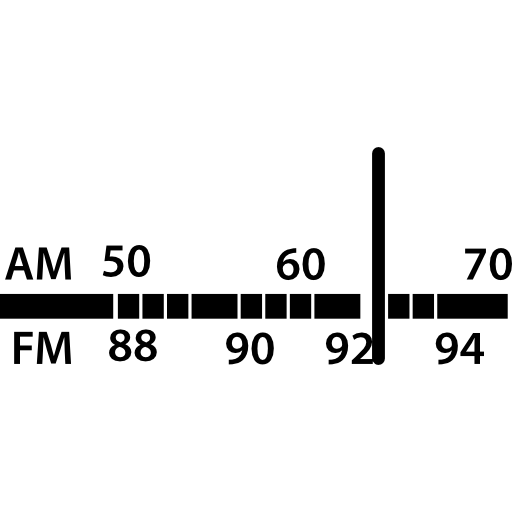
\includegraphics[height=.7\paperheight]{misc/radio-am-und-fm-tuner.png}\hfil}\vfil}
	}
	\frame{
		\frametitle{Fine Tuning!}
		\begin{mdframed}[tikzsetting={draw=white,fill=white,fill opacity=0.8,
				line width=0pt},backgroundcolor=none,leftmargin=0,
			rightmargin=150,innertopmargin=4pt,roundcorner=10pt]
			\tableofcontents[currentsection,sections={1-4},hideothersubsections]
		\end{mdframed}
	}
}

%<a href="https://www.flaticon.com/de/kostenlose-icons/radio" title="radio Icons">Radio Icons erstellt von Freepik - Flaticon</a>

%%%%%%%%%%%%%%%%%%%%%%%%%%%%%%%%%%%%%%%%%%%%%%%%%%%%%%%%%%%%%%%%%%%%%%%%%%%%%%%%
\begin{frame}
	\frametitle{What is this about?}
	\begin{question}[Questions]
		\begin{itemize}
			\item What if I really need to submit \textbf{\textsc many} jobs?
	        \item Will crash the cluster?
	        \item My admins report a slow accounting DB. How do I cope with that?
		\end{itemize}
	\end{question}
	\begin{docs}[Objectives]
		\begin{enumerate}
			\item Learning how throttle job submission with \Snakemake{}.
			\item Knowing how to limit the status request from \Snakemake to SLURM.
		\end{enumerate}
	\end{docs}
\end{frame}

%%%%%%%%%%%%%%%%%%%%%%%%%%%%%%%%%%%%%%%%%%%%%%%%%%%%%%%%%%%%%%%%%%%%%%%%%%%%%%%%%
\begin{frame}[fragile]
	\frametitle{Limiting Job Submission Rates}
	\begin{docs}
		We can limit the number of jobs submitted per second with the \altvberb{--max-jobs-per-second} flag.\newline
		\emph{However}, this is only necessary, when dealing with an enormous load of jobs ($\gg$ 1.000 -- 10.000 jobs)\newline\pause
		The default is 10 per second.
	\end{docs}
    \begin{lstlisting}[language=Bash, style=Shell]
$ snakemake --max-job-per-second=0.1
   \end{lstlisting}	
   The value may be a fraction (here: 1 job per ten seconds). Or simply
   \begin{lstlisting}[language=Bash, style=Shell]
$ snakemake --max-job-per-second=5
   \end{lstlisting}
   which would half the submission rate (5 instead of 10)
\end{frame}

%%%%%%%%%%%%%%%%%%%%%%%%%%%%%%%%%%%%%%%%%%%%%%%%%%%%%%%%%%%%%%%%%%%%%%%%%%%%%%%%%
\begin{frame}[fragile]
	\frametitle{Limiting Job Status Queries}
	\begin{docs}
		The SLURM executor plugin has its own limiter and ensures that the accounting data base is not overwhelmed.\newline
		The \altverb{--max-status-checks-per-second} flag allows us to throttle the number of status queries per second.\newline
		The default is at 10. -- Usefull for local jobs, only.
    \end{docs}
\end{frame}